\section{Entropy} \label{sec:shannon_entropy}

We now introduce the concept of entropy as a measure of uncertainty of a random variable. While the worst-case entropy $H_{wc}$, discussed previously, provides a lower bound based solely on the set's cardinality (effectively assuming fixed-length codes or a uniform probability distribution over the elements), Shannon entropy offers a more refined measure. It accounts for the actual probability distribution of the elements, quantifying the \emph{average} uncertainty or information content associated with the random variable. A deeper explanation can be found in standard texts such as \cite{han2002mathematics,navarro2016compact,ElementsofInformationTheory}.

\begin{definition}[Entropy of a Random Variable]\label{def:entropy}
    Let $X$ \marginpar{This is also known as Shannon entropy, named after Claude Shannon, who introduced it in his seminal work \cite{Shannon1948}}be a random variable taking values in a finite alphabet $\mathcal{X}$ with the probabilistic distribution $P_X(x)= \text{Pr}\{X=x\}~(x\in\mathcal{X})$. Then, the entropy of $X$ is defined as
    \begin{equation*}
        H(X) = H(P_X) \myeq E_{P_x} \{-\log P_X(x)\} = -\sum_{x\in\mathcal{X}} P_X(x)\log P_X(x)
    \end{equation*}
\end{definition}
Here, $E_{P_X}[\cdot]$ denotes the expectation with respect to the probability distribution $P_X$. The logarithm is taken to base 2, and entropy is expressed in bits. From the definition, it follows that the entropy of a discrete random variable is always non-negative\footnote{The entropy is zero if and only if $X$ is deterministic, i.e., $P_X(x)=1$ for some single value $x=c$.}. \label{foot:entropy_nonneg}.

\begin{example}[Toss of a fair coin]
    Let $X$ be a random variable representing the outcome of a fair coin toss, with $\mathcal{X}=\{Heads, Tails\}$. The probability distribution is $P_X(\text{Heads}) = P_X(\text{Tails}) = \frac{1}{2}$. The entropy of $X$ is:
    \begin{equation*}
        H(X) = -\frac{1}{2}\log_2\frac{1}{2} - \frac{1}{2}\log_2\frac{1}{2} = -\frac{1}{2}(-1) - \frac{1}{2}(-1) = 1 \text{ bit}
    \end{equation*}
    This result aligns with the intuition that one bit is required to convey the outcome of a fair coin toss.
\end{example}

\begin{remark}
    By convention, $H(X)$ denotes the entropy of the random variable $X$. It is important to note that entropy is not a function of the random variable itself, but rather a functional of its probability distribution $P_X$. It depends only on the probabilities of the values, not the values themselves.
\end{remark}

The entropy $H(X)$ quantifies the average uncertainty associated with the random variable $X$. It can be interpreted as the average amount of information (in bits) gained upon observing an outcome of $X$, or equivalently, the minimum average number of bits required to encode the outcomes of $X$ using an optimal compression scheme.

\subsection{Properties}
Having introduced the entropy for a single random variable $X$, we now consider the case of two random variables $X$ and $Y$. To quantify the total uncertainty associated with the pair $(X,Y)$ considered together, we define the joint entropy:

\begin{definition}[Joint Entropy]\label{def:joint_entropy}
    Let $(X,Y)$ be a pair of discrete random variables $(X,Y)$ with a joint distribution $P_{XY}(x,y) = \text{Pr}\{X=x,Y=y\}$. The joint entropy of $(X,Y)$ is defined as
    \begin{equation*}\label{eq:joint_entropy}
        H(X,Y) = H(P_{XY}) = -\sum_{x\in\mathcal{X}}\sum_{y\in\mathcal{Y}} P_{XY}(x,y)\log P_{XY}(x,y)
    \end{equation*}
\end{definition}
This definition extends naturally to the joint entropy of $n$ random variables $(X_1,X_2,\ldots,X_n)$ as $H(X_1,\ldots, X_n)$.

We also define the conditional entropy $H(Y|X)$, which measures the remaining uncertainty about $Y$ when $X$ is known. It is the expected value of the entropies of the conditional distributions $P_{Y|X}(y|x)$, averaged over $X$.

Often, it's helpful to conceptualize the relationship between $Y$ and $X$ in terms of information transmission. Given $X=x$, the conditional probability $P_{Y|X}(y|x) = \text{Pr}\{Y=y|X=x\}$ describes the likelihood of observing $Y=y$. The collection of these conditional probabilities for all $x \in \mathcal{X}$ and $y \in \mathcal{Y}$ defines a statistical relationship often referred to as a \emph{channel} with \emph{input alphabet} $\mathcal{X}$ and \emph{output alphabet} $\mathcal{Y}$.

\begin{definition}[Conditional Entropy]\label{def:conditional_entropy}
    Let $(X,Y)$ be a pair of discrete random variables with a joint distribution $P_{XY}(x,y) = \text{Pr}\{X=x,Y=y\}$. The conditional entropy of $Y$ given $X$ is defined as
    \begin{align*}
        H(Y|X) & = H(W | P_X) \myeq \sum_x P_X(x)H(Y|x)                                                       \\
               & = \sum_{x \in \mathcal{X}} P_X(x) \Big\{ -\sum_{y \in \mathcal{Y}} W(y|x) \log W(y|x) \Big\} \\
               & = -\sum_{x\in\mathcal{X}}\sum_{y\in\mathcal{Y}} P_{XY}(x,y)\log W(y|x)                       \\
               & = E_{P_{XY}} \{ -\log W(Y|X) \}
    \end{align*}
\end{definition}

Since entropy is non-negative, and $H(Y|X)$ is an average of non-negative entropies $H(Y|X=x)$, conditional entropy is also non-negative: $H(Y|X) \ge 0$. Furthermore, $H(Y|X) = 0$ if and only if $Y$ is completely determined by $X$ (i.e., $Y=f(X)$ for some deterministic function $f$ with probability one).

The relationship between joint and conditional entropy is established by the chain rule.

\begin{theorem}[Chain Rule]\label{thm:chain_rule}
    Let $(X,Y)$\marginpar{This is also known as additivity of entropy.} be a pair of discrete random variables with a joint distribution $P_{XY}(x,y)$. Then, the joint entropy of $(X,Y)$ can be expressed as
    \begin{equation*}
        H(X,Y) = H(X) + H(Y|X)
    \end{equation*}
\end{theorem}
\begin{proof}
    From the definition of conditional entropy (\ref{def:conditional_entropy}), we have
    \begin{align*}
        H(X,Y) & = -\sum_{x,y} P_{XY}(x,y) \log W(y|x)                                        \\
               & = -\sum_{x,y} P_{XY}(x,y) \log \frac{P_{XY}(x,y)}{P_X(x)}                    \\
               & = -\sum_{x,y} P_{XY}(x,y) \log P_{XY}(x,y) + \sum_{x,y} P_{X}(x) \log P_X(x) \\
               & = H(X,Y) + H(X)
    \end{align*}
    Where we used the relation
    \begin{equation*}
        W(y|x) = \frac{P_{XY}(x,y)}{P_X(x)}
    \end{equation*}
    When $P_X(x) \neq 0$.
\end{proof}

\begin{corollary}
    \begin{equation*}
        H(X, Y|Z) = H(X|Z) + H(Y|X,Z)
    \end{equation*}
\end{corollary}
\begin{proof}
    The proof is analogous to the proof of the chain rule.
\end{proof}

\begin{corollary}
    \begin{align*}
        H(X_1, X_2, \ldots, X_n) & = H(X_1) + H(X_2|X_1) + H(X_3|X_1, X_2) \nonumber \\
                                 & + \ldots + H(X_n|X_1, X_2, \ldots, X_{n-1})
    \end{align*}
\end{corollary}
\begin{proof}
    We can apply the two-variable chain rule in repetition obtain the result.
\end{proof}

\subsection{Mutual Information}
Having defined measures for the uncertainty of individual variables ($H(X)$), pairs ($H(X,Y)$), and conditional uncertainty ($H(Y|X)$), we can quantify the amount of information that one variable provides about another. This is the mutual information, $I(X;Y)$. It represents the reduction in uncertainty about $X$ obtained by learning the value of $Y$, or vice versa. Figure \ref{fig:mutual_information} provides a visual representation.

\begin{definition}[Mutual Information]\label{def:mutual_information}
    Let $(X,Y)$ be a pair of discrete random variables with a joint distribution $P_{XY}(x,y)$. The mutual information between $X$ and $Y$ is defined as
    \begin{equation}
        I(X;Y) = H(X) - H(X|Y)
    \end{equation}
\end{definition}
Using the chain rule (\ref{thm:chain_rule}), we can rewrite it as
\begin{align}
    I(X;Y) & = H(X) - H(X|Y) \nonumber                                           \\
           & = H(X) + H(Y) - H(X,Y)                                              \\
           & = -\sum_x P_X(x)\log P_X(x) - \sum_y P_Y(y)\log P_Y(y) \nonumber    \\
           & \quad + \sum_{x,y} P_{XY}(x,y)\log P_{XY}(x,y)                      \\
           & = \sum_{x,y} P_{XY}(x,y)\log \frac{P_{XY}(x,y)}{P_X(x)P_Y(y)}       \\
           & = E_{P_{XY}} \left\{ \log \frac{P_{XY}(x,y)}{P_X(x)P_Y(y)} \right\}
\end{align}
It follows immediately that the mutual information is symmetric, $I(X;Y) = I(Y;X)$.

\begin{figure}[h!]
    \centering
    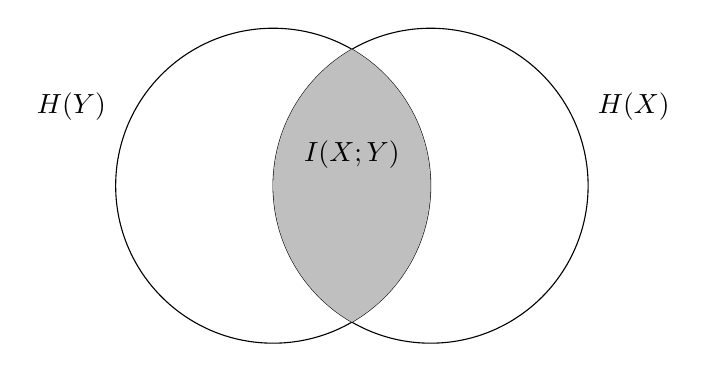
\begin{tikzpicture}
        % Define the circles
        \def\radius{2cm}
        \def\dist{2cm}
        \coordinate (center1) at (0,0);
        \coordinate (center2) at (\dist,0);

        % Draw circles
        \draw (center1) circle [radius=\radius];
        \draw (center2) circle [radius=\radius];

        % Color intersection
        \begin{scope}
            \clip (center1) circle (\radius);
            \fill[lightgray] (center2) circle (\radius);
        \end{scope}

        % Label intersection
        \coordinate (intersection) at (\dist/2,0);
        \node at (intersection) [below, above=0.1cm] {$I(X;Y)$};

        % Move labels outside
        \node at (center1) [above=1cm, left=2cm] {$H(Y)$};
        \node at (center2) [above=1cm, right=2cm] {$H(X)$};
    \end{tikzpicture}
    \caption{Mutual information between two random variables $X$ and $Y$.\label{fig:mutual_information}}
\end{figure}

\subsection{Fano's inequality}

Information theory provides fundamental limits on data processing tasks, including compression and inference. It allows us to establish lower bounds on the probability of error when estimating one random variable based on observations of another. Fano's inequality relates the conditional entropy $H(X|Y)$ to the probability of error when estimating $X$ from $Y$. Recall that $H(X|Y) = 0$ if and only if $X$ is a function of $Y$, meaning $X$ can be determined from $Y$ with zero error. Fano's inequality bounds the error probability when $H(X|Y) > 0$.

\begin{theorem}[Fano's Inequality]\label{thm:fano_inequality}
    Let $X$ and $Y$ be two discrete random variables with $X$ taking values in some discrete alphabet $\mathcal{X}$, we have
    \begin{equation*}
        H(X|Y) \leq \text{Pr}\{X \neq Y\} \log (|\mathcal{X}|-1) + h(\text{Pr}\{X \neq Y\})
    \end{equation*}
    where $h(p) = -p\log p - (1-p)\log(1-p)$ is the binary entropy function.
\end{theorem}
\begin{proof}
    Let $Z$ be a random variable defined as follows:
    \begin{equation*}\label{eq:random_variable_Z}
        Z = \begin{cases}
            1 & \text{if } X \neq Y \\
            0 & \text{if } X = Y
        \end{cases}
    \end{equation*}
    We can then write
    \begin{align} \label{eq:entropy_decomposition}
        H(X|Y) & = H(X|Y) + H(Z|XY) = H(XZ|Y) \nonumber \\
               & = H(X|YZ) + H(Z|Y) \nonumber           \\
               & \leq H(X|YZ) + H(Z)
    \end{align}
    The last inequality follows from the fact that conditioning reduces entropy. We can then write
    \begin{equation} \label{eq:entropy_decomposition2}
        H(Z) = h(\text{Pr}\{X \neq Y\})
    \end{equation}
    Since $\forall y \in \mathcal{Y}$, we can write
    \begin{equation*}
        H(X | Y =y, Z =0) =0
    \end{equation*}
    and
    \begin{equation*}
        H(X| Y = y, Z = 1) \leq \log(|\mathcal{X}|-1)
    \end{equation*}
    Combining these results, we have
    \begin{equation} \label{eq:entropy_decomposition3}
        H(X | YZ) \leq \text{Pr}\{X \neq Y\} \log (|\mathcal{X}|-1)
    \end{equation}
    From equations \ref{eq:entropy_decomposition}, \ref{eq:entropy_decomposition2} and \ref{eq:entropy_decomposition3}, we have Fano's inequality.
\end{proof}
Fano's inequality thus provides a tangible link between the conditional entropy $H(X|Y)$, which quantifies the remaining uncertainty about $X$ when $Y$ is known, and the minimum probability of error achievable in any attempt to estimate $X$ from $Y$. This inequality, along with the foundational concepts of entropy, joint entropy, conditional entropy, and mutual information introduced throughout this section, establishes a robust theoretical framework. These tools are not merely abstract measures; they allow us to quantify information, understand dependencies between data sources, and ultimately, to delineate the fundamental limits governing how efficiently data can be represented and compressed. Understanding these limits is essential as we go deeper into specific encoding techniques.
